\chapter{Introduzione}

\section{Motivazione}
% Spiegare il perchè l'ho fatto Dati importanti, piccole e medie imprese devono sfruttare software opensource disponibili a tutti che permetto di passare da una frase experimental a production ready

Le piccole e medie imprese sono sempre più informatizzate e dipendenti da servizi informatici per poter continuare a lavorare. Per questo motivo scoprire e analizzare il traffico anomalo che passa sulle reti aziendali è sempre più importante, il nostro obiettivo è farlo ad un basso costo, senza aggiungere applicativi che richiedono molta potenza di calcolo o di banda ai router che compongono la rete. Punteremo a scoprire le anomalie nei dati di rete di singoli flussi e dati aggregati analizzando i dati su un server aggiuntivo che si occuperà anche di mitigare l'attacco informando i router sui flussi da bloccare.
Gli attacchi maggiormente presi in considerazione in questa tesi sono gli attacchi di Distributed Denial of Service, ma i suoi principi possono essere applicati anche ad altre tipologie di anomalie.
% problema delle botnets
Inoltre raccogliere informazioni sull'utilizzo della rete può portare anche alla risoluzioni di problemi non derivanti da attacchi.

\section{Scenario}
\begin{figure}[]
    \label{fig:scenario}
    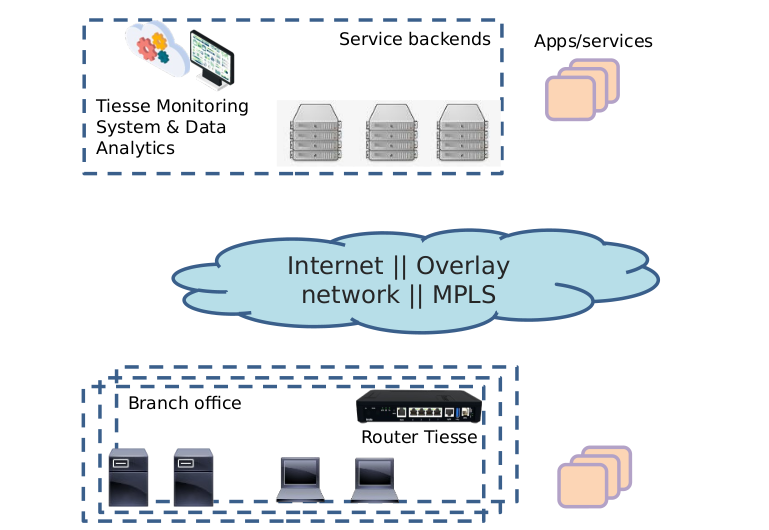
\includegraphics[width=\hsize]{images/introduzione/scenario_2.png}
    \caption{Scenario rete Tiesse e clienti}
    \centering
\end{figure}

Per fare questa tesi abbiamo preso in considerazione un tipico scenario aziendale, in cui esiste una sede centrale, ben protetta e su cui sono ospitati i servizi dell'azienda e tante sedi periferiche: uffici, negozi o altro, collegati ai servizi della sede centrale tramite un overlay MPLS o una VPN.
Le sedi periferiche sono quelle più esposte sotto l'aspetto della sicurezza (todo: magari spiegare i motivi. anche solo perchè sono tante e spesso non ci sono i responsabili dell it in sede), per questo motivo il nostro obiettivo è quello di proteggere i servizi aziendali e la rete centrale dai pc connessi alle reti degli uffici.
L'organizzazione di Tiesse e di molti suoi clienti è caratterizzata da questo scenario \ref{fig:scenario}, per questo motivo le prove da me effettuate si basano sull'analisi del traffico proveniente dall'ufficio di Torino e mirano a proteggere i servizi aziendali presenti nella sede centrale di Ivrea a cui l'ufficio di Torino è collegato tramite una VPN.
Un altro caso possibile di utilizzo di questa soluzione è la distribuzione dei servizi in cloud, in cui l'azienda non ha il controllo dell'infrastruttura di rete.


% todo: sostituire servizi con applicativi aziendali

\begin{figure}[]
    \label{fig:scenario_2}
    %https://lucid.app/lucidchart/8119c7e9-e2e1-4dbb-b55f-bebf6c97af2d/edit?beaconFlowId=3612F8C43004D8D2&page=0_0#
    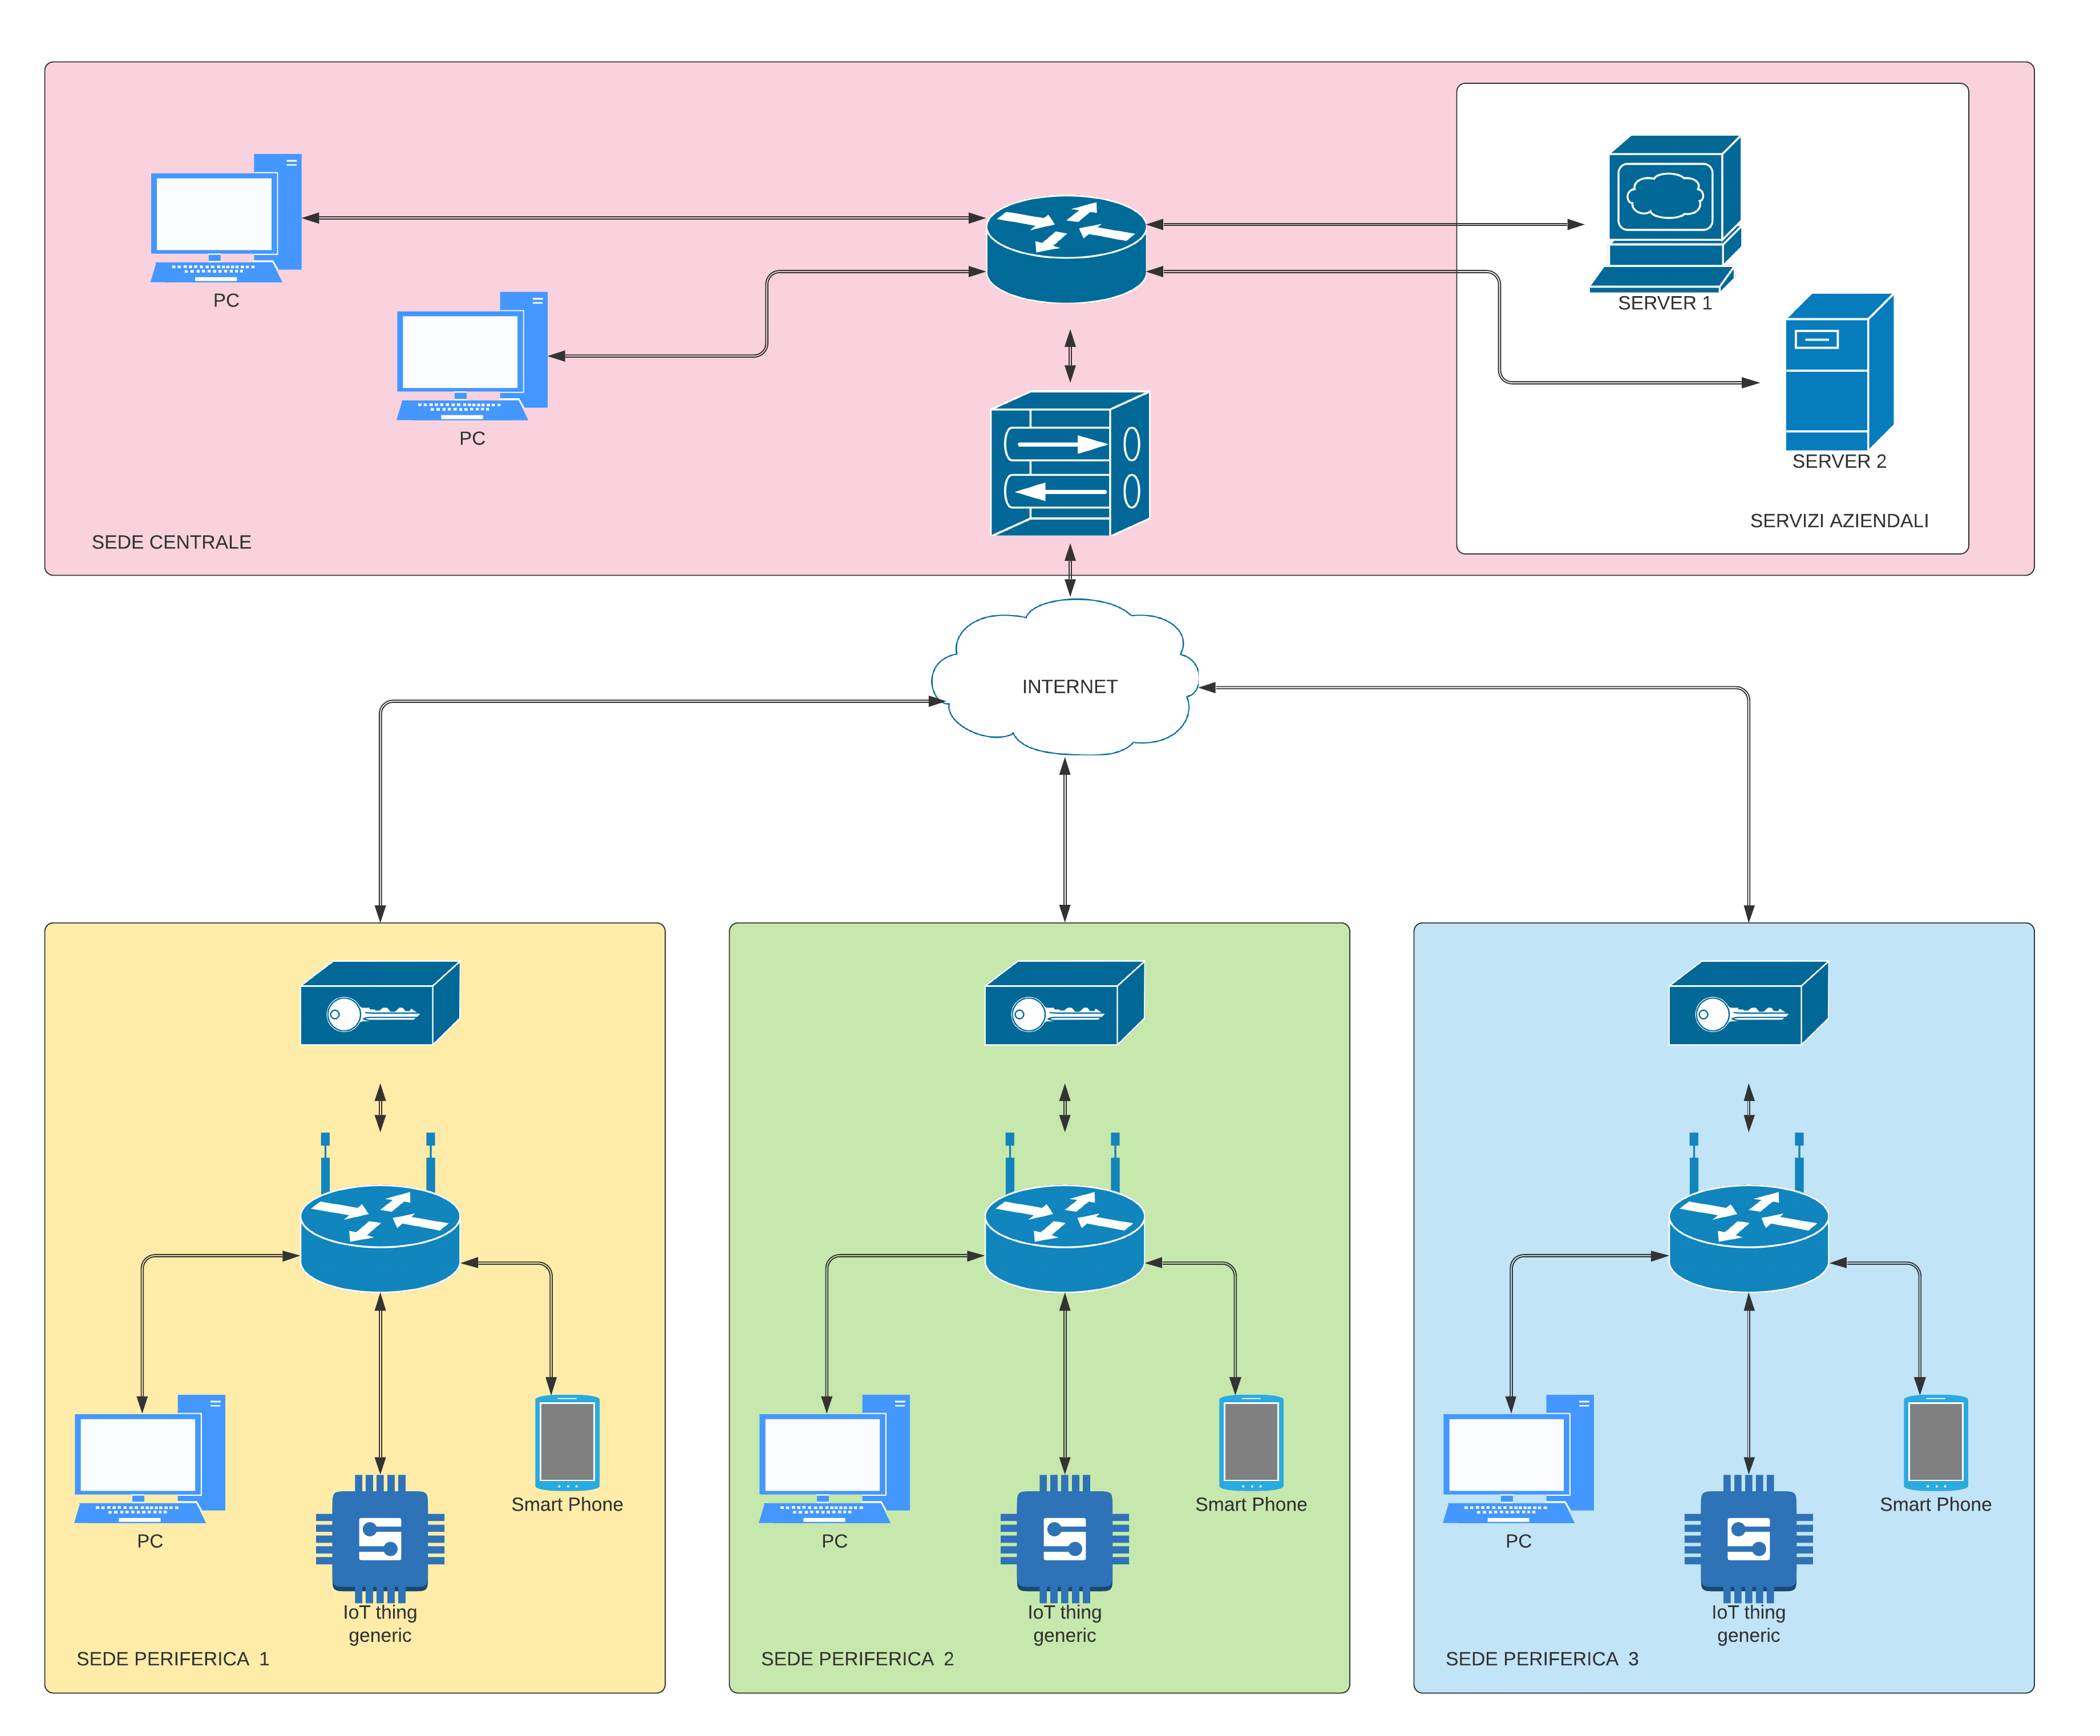
\includegraphics[width=\hsize]{images/introduzione/scenario.png}
    \caption{Scenario rete Tiesse e clienti}
    \centering
\end{figure}




\section{Gli attacchi DDoS}

Gli attacchi di Denial of Service (DoS) sono degli attacchi nel campo della sicurezza informatica che mirano a interrompere la fruizione di un servizio, fornito da un host connesso a internet, da parte di utenti legittimi. L'attacco ha l'obiettivo di esaurire le risorse dell'host in modo da non consentirgli di erogare le risposte ai richiedenti.
Nel caso in cui la sorgente del traffico che mira a creare disservizi non sia unica, si parla di attacchi di denial of service distribuiti (Distributed Denial of Service).

\subsection{Tipologia di attacchi DDoS}
    
Gli attacchi DDoS possono essere suddivisi in due categorie principali in base al loro funzionamento. La prima si basa sul mandare alla vittima pacchetti malformati in grado di sfruttare un bug ana falla a livello applicativo. La seconda categoria invece si basa su tecniche per colpire l'infrastruttura del servizio, per il funzionamento di questa tecnica vengono usati uno o entrambi i seguenti metodi: uno punta sull'interruzione della connessione di rete grazie all'esaurimento della banda o della capacità di processamento dei router o di entrambe, nel secondo caso l'obiettivo dell'attaccante è di esaurire le risorse (es. sockets, CPU, memoria) del server che ospita il servizio \cite{ddos_survey_1}.

\begin{figure}[h]
    % todo: capire come gestire citazioni imsmagini a livello di copyright
    %  e capire come funzionano le label per richiamare le immagini
    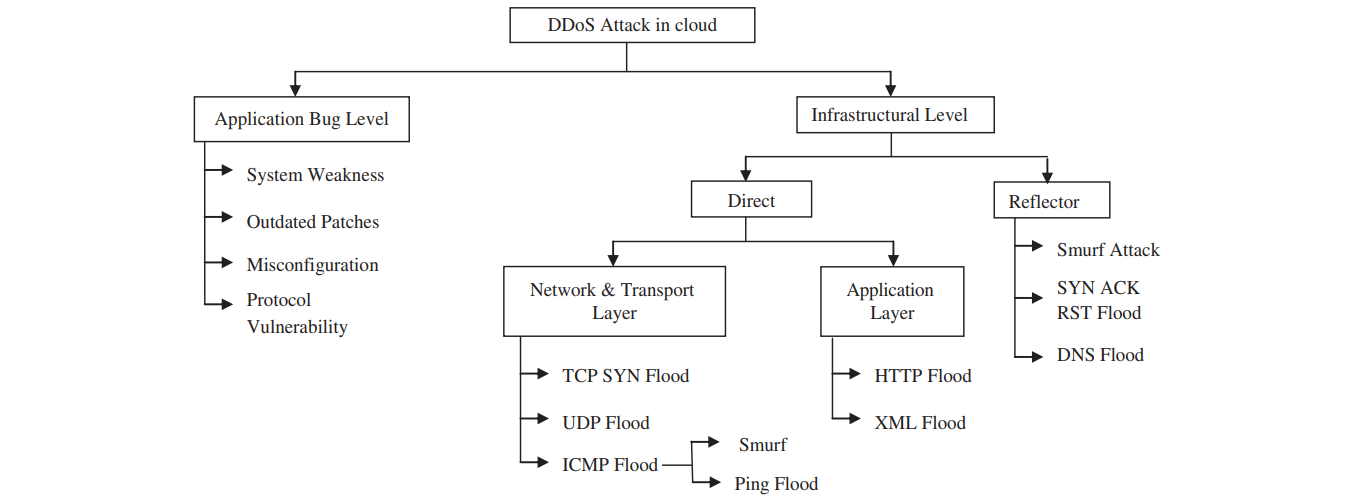
\includegraphics[width=\hsize]{images/introduzione/tipologie_ddos.png}
    \caption{Tipologie di attacchi DDoS \cite{ddos_survey_3}}
    \centering
\end{figure}

L'obiettivo di questa sarà concentrato sul rilevamento e la mitigazione della seconda categoria di attacchi, basata sull'esaurimento delle risorse.

\subsubsection{Attacchi basati sul flooding}

\begin{figure}[h]
    % todo: capire come gestire citazioni immagini a livello di copyright
    %  e capire come funzionano le label per richiamar le immagini
    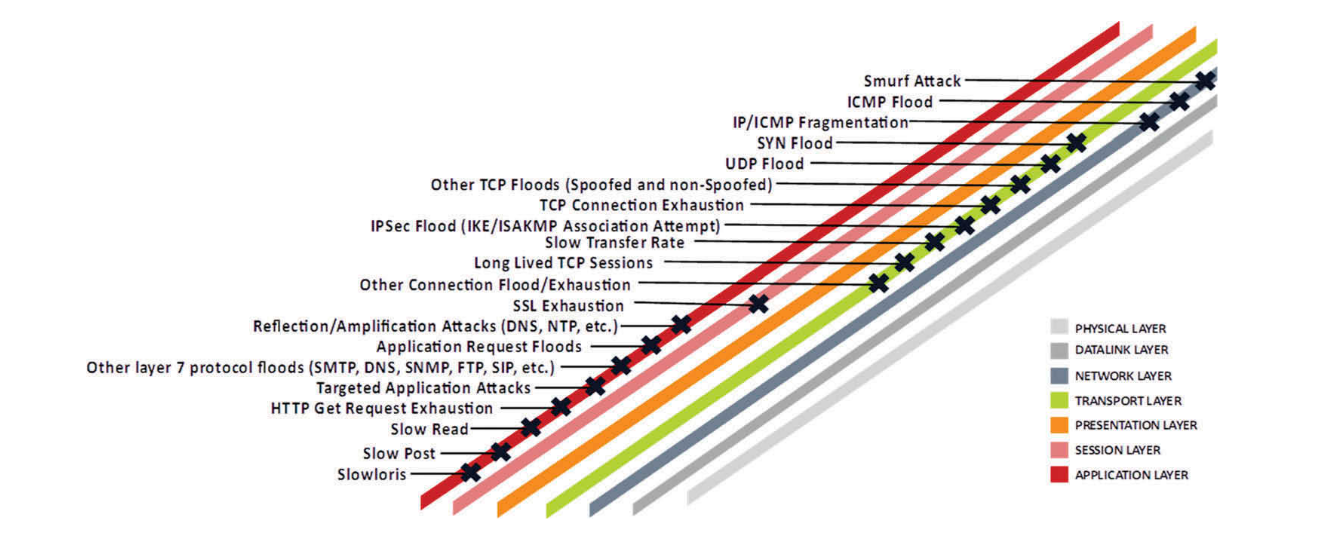
\includegraphics[width=\hsize]{images/introduzione/attacchi_per_livello.png}
    \caption{Attacchi per livello \cite{ddos_survey_4}}
    \centering
\end{figure}

\paragraph{Network/transport-level DDoS flooding attacks} % todo: rivedere titolo
Gli attacchi di denial of service che mirano ad esaurire le risorse di rete si basano sull'invio di molti pacchetti che consumino totalmente la banda della vittima, queste tipologia di attacco può essere effettuata in maniera diretta: \emph{flooding attacks} e \emph{protocol exploitation attacks}, nel primo caso la vittima viene inondata di pacchetti (UDP flood, ICMP flood, DNS flood, VoIP flood an etc.), in questo caso la banda aggregata in uscita di tutti gli attaccanti deve essere superiore a quella del servizio che si vuole interrompere, nel secondo caso vengono sfruttane delle caratteristiche dei protocolli della vittima in modo da consumare una grande quantità di risorse (es. TCP SYN flood, TCP SYN-ACK flood, RST/FIN flood e ecc).

Gli attacchi che non vengono che non vengono effettuati in maniera diretta invece sfruttano la riflessione o l'amplificazione: nella \emph{Reflection-based flooding attacks} chi attacca manda un particolare pacchetto, indirizzandolo ad un riflettore e questo riflettore manda le sue risposte alla vittima, in modo da esaurire le risorse della vittima. Un esempio di questo attacco sono lo Smurf e il Fraggle, nel primo vengono mandati ICMP Echo Request ad una sottorete, usando come ip di destinazione l'indirizzo broadcast e con ip spoofing, specificando come ip sorgente l'ip della vittima, causando la risposta di tutti gli host verso l'indirizzo della vittima \cite{ddos_survey_2}.
Gli \emph{Amplification-based flooding attacks} sfruttano servizi che restituiscono risposte più grandi della richiesta ricevuta, un esempio è il DNS amplification, che riesce a moltiplicare dalle 30 alle 50 volte\cite{imperva_amplification} la banda in uscita dell'attaccante, il suo funzionamento si basa sull'utilizzo dell'ip spoofing mandando un pacchetto con indirizzo ip sorgente della vittima, così il servizio DNS risponderà alla vittima con un flood di pacchetti di dimensioni maggiori \cite{ddos_survey_1}. Lo stesso principio è sfruttato anche dal NTP amplification che può amplificare il traffico con un rapporto tra 20:1 e 200:1, arrivando in alcuni casi a 556:1 \cite{imperva_amplification}. 

% todo: Amplification-based flooding attack, negli attacchi di rete: qua non so giustificarla bene pagina 3 \cite{ddos_survey_1}
% qua parla bene del fattore di moltiplicazione degli attacchi https://www.imperva.com/blog/ntp-flood-explained/

\paragraph{Application-level DDoS flooding attacks} % todo: rivedere titolo
% qua taglio un po' corto sugli attacchi applicativi perchè approfondirò maggiormente quelli di rete
Gli attacchi DDoS al livello applicativo hanno lo scopo di terminare le risorse del server(sockets, cpu, memory, disk/db bandwidth, I/O bandwidth) e di solito usano meno banda, rispetto gli attacchi di alla rete, per questo motivo è anche più difficile identificarli. Le tecniche utilizzate sono simili alle precedenti. Degli esempi sono l'HTTP flooding che grazie con molte richieste, obbliga il server a produrre risposte che possono essere computazionalmente pesanti, oppure l'SQL Injection per imporre un lock sul database e bloccare il funzionamento dell'applicazione, altri attacchi possono essere l'HTTP fragmentation, lo slowpost attack, slowreading attack e lo slowloris attack, tutte che mirano a mantenere la connessione aperta mandando o ricevendo pochi dati per volta \cite{ddos_survey_1}.
Gli attacchi di tipo applicativo possono essere molto eterogenei e non possono essere mitigati a livello di rete/trasporto, per questo motivo questa tesi prenderà in considerazione solo gli attacchi trattati al paragrafo precedente.

\paragraph{DDoS con obiettivo la riduzione della qualità del servizio}

% parlare anche di attacchi a basso rate, ma da molte fonti che portano ad un grande risultato finale \cite{ddos_survey_4,ddos_survey_3} pagina 38, rendendolo difficile da indentificare

L'unico obiettivo possibile degli attacchi DDoS non è la sola interruzione del servizio, ma un altro risultato è la degradazione del servizio, consumando una parte di risorse destinate agli utenti legittimi e creando loro ritardi nelle risposte. Questo risultato può essere raggiunto utilizzando dei packet rate più bassi, e di conseguenza meno rilevabili o dei rate variabili \cite{ddos_survey_3, ddos_survey_4}.

\subsection{Vittime attacchi DDoS}

I target degli attacchi DDoS possono variare molto da un utente domestico ad un governo \cite{ddos_motivations}.

% todo: introduzione: qua potrei nominare delle statistiche sugli attacchi con la distribuzione delle vittime

Per capire maggiormente chi possono essere le vittime di un attacco bisogna analizzare le motivazioni che spingono gli attaccanti e con le diverse motivazioni può cambiare anche la portata dell'attacco. Per semplicità possiamo dividere gli incentivi di un attacco in cinque principali categorie \cite{ddos_survey_1}\cite{ddos_motivations}:

\begin{itemize}
    \item Beneficio economico o finanziario: sono gli attacchi che riguardano principalmente le aziende, sono considerati i più pericolosi e difficili da fermare, perché mirano ad ottenere benefici finanziari dagli attacchi. I creatori dell'attacco normalmente sono persone con esperienza.
    \item Vendetta: questa Tipologia di attacchi sono mesi in atto da persone, solitamente con uno scarso livello tecnico, a fronte di un'apparente ingiustizia percepita.
    \item Credo ideologico: alcuni attaccanti si trovano ad effettuare attacchi contro degli obiettivi per motivi ideologici. È una motivazione di attacco meno comune delle altre, ma può portare ad attacchi di grande entità. % todo: valutare se mettere esempi attacchi tipo cnn 2008, wikileaks 2010 e iran 2009
    \item Sfida intellettuale: gli utenti che sviluppano attacchi per questa motivazione che vogliono imparare e sperimentare a lanciare attacchi, spesso sono giovani appassionati di hacking che grazie alla facilità con cui si possono affittare botnets o utilizzare semplici tool riescono ad effettuare con successo DDoS.
    \item Cyberwarfare: gli attaccanti di questa categoria appartengono ad organizzazioni terroristiche o militari di un paese e sono politicamente motivati ad attaccare risorse critiche di un altro paese. Un grande numero di risorse viene usato per questa tipologia di attacco e può paralizzare le infrastrutture critiche di un paese, portando ad un grave impatto economico.
\end{itemize}


\subsection{Diffusione attacchi DDoS}

Nel mondo gli attacchi a fine 2020 la quasi totalità degli attacchi DDoS proveniva da botnets, con target principali in Cina e negli Stati Uniti. Le tipologie di attacco maggiormente utilizzate sono guidate dal \emph{Syn Flood} che copre più del 90\% della totalità degli attacchi, seguito da \emph{ICMP flooding} e \emph{UDP flooding} \cite{ddos_kaspersky} \cite{ddos_kaspersky_q3_2020}.

\begin{figure}[h]
    % todo: capire come gestire citazioni immagini a livello di copyright
    %  e capire come funzionano le label per richiamar le immagini
    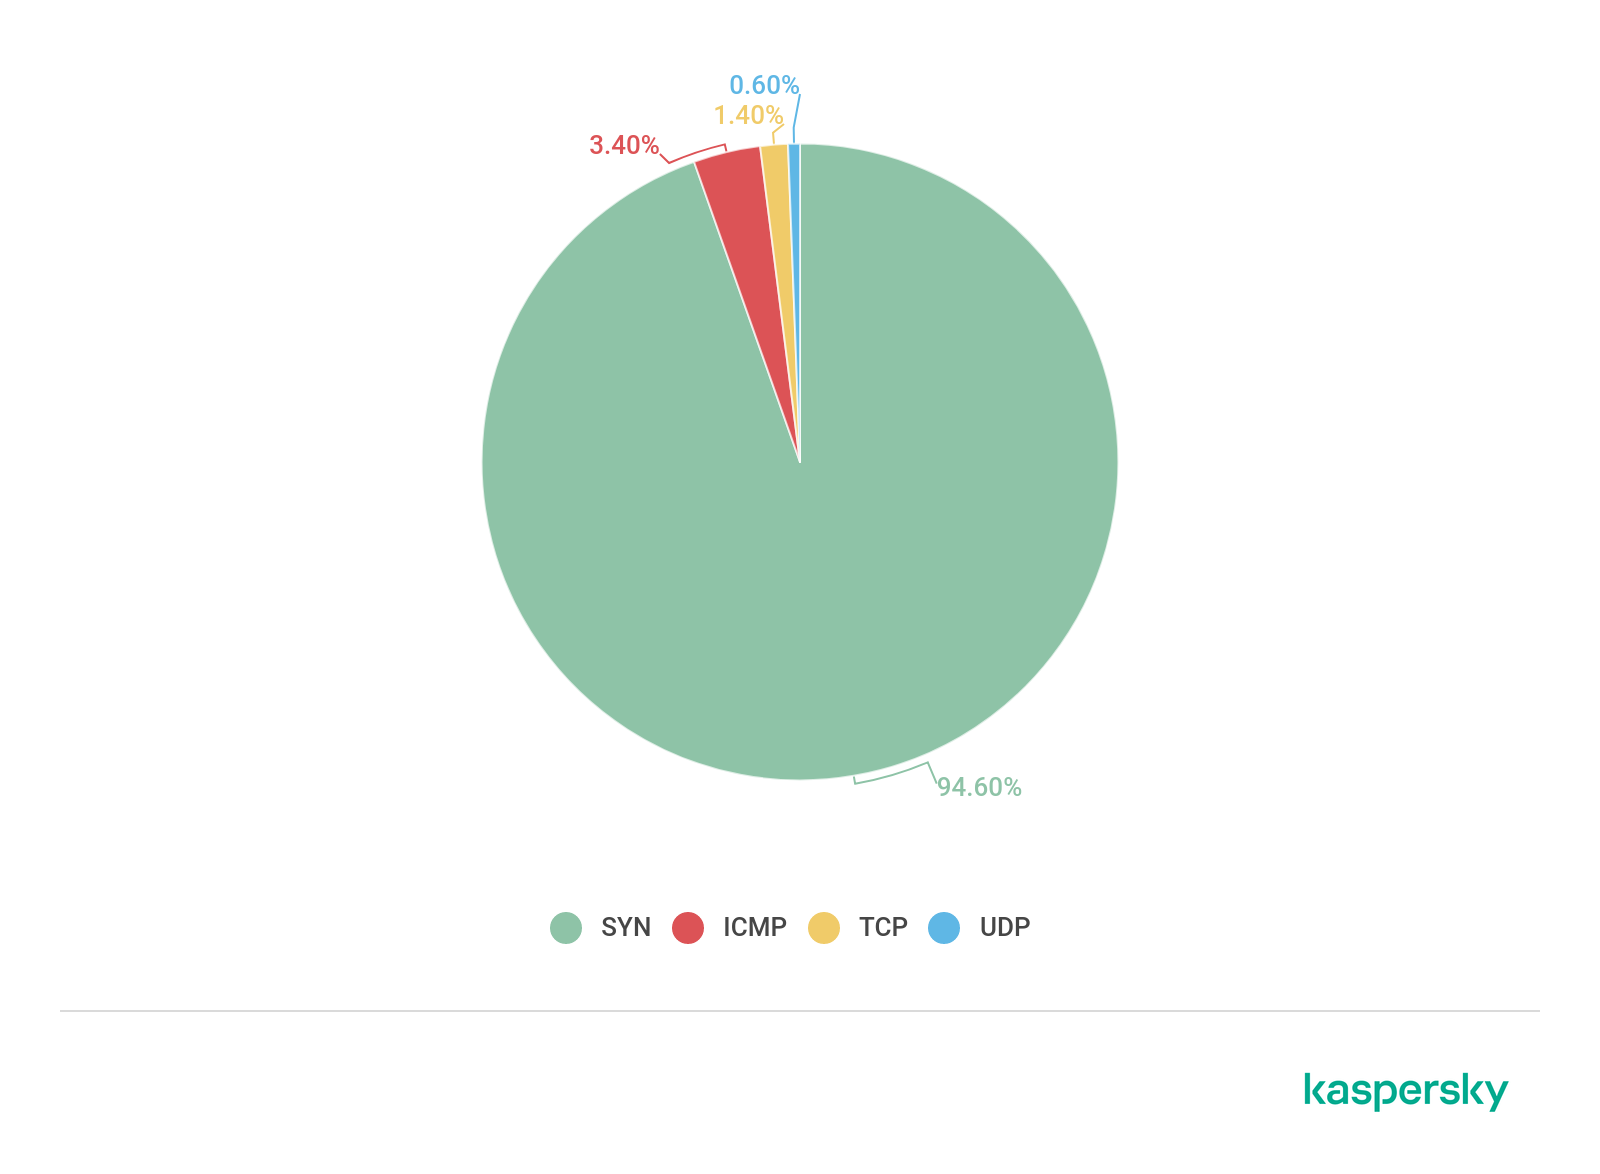
\includegraphics[width=\hsize]{images/introduzione/07-en-ddos-report-q3-2020-chrarts.png}
    \caption{Distribuzione di attacchi DDoS per tipologia, Q3 2020 \cite{ddos_kaspersky_q3_2020}}
    \centering
\end{figure}

\subsubsection{Attacchi DDoS famosi}

%todo: qua parla del flood dns https://www.cloudflare.com/it-it/learning/ddos/dns-flood-ddos-attack/

Prova prova

% todo: parlare di botnet => MIRAI


\subsubsection{Attacchi basati su botnets}

Gli attacchi basati su botnets sono un grande problema per l'implementazione di sistemi anti-DDoS perché un grande numero di ``zombie'' rende l'attacco più distruttivo e spesso utilizzano ip spoofing, il che rende più difficile il tracciamento all'indietro per determinare i bot. \cite{ddos_survey_1}
% todo: qui dovrei magari differenziare le botnet controllate direttamente e indirettamente e dilungarmi meno, magari nominare le tre fasi degli attacchi \cite{ddos_motivations} pagina 5 \cite{ddos_survey_4} pagina 37
I bot possono essere controllati dell'artefice dell'attacco tramite tre architetture \cite{ddos_survey_4}: % pagina 46
\begin{itemize}
    \item IRC-based: architettura client-server in cui ad ogni server si possono collegare centinaia di dispositivi, utilizza un protocollo testuale e utilizzando porte non standard rende molto difficile il riconoscimento del comando per lanciare un DDoS, il quale si può nascondere facilmente nel grande traffico dei server IRC, ma il singolo server a cui si connettono tutti i client può essere considerato un single point of failure.
    \item Web based: ogni bot scarica periodicamente delle informazioni tramite una richiesta web ad un server, i comandi di questa tipologia di controllo sono i più difficili da tracciare.
    \item P2P based:le moderne botnet utilizzano una struttura più robusta e flessibile, invece di avere un singolo server centrale chi è al controllo della botnet manda un comando in broadcast a tutti gli agent, questo lo rende più affidabile e l'eliminazione di un agent non rende la rete non funzionante, ma rende la rete più difficile da mantenere e la scoperta di un agent può mostrare tutti gli altri. 
\end{itemize}

\begin{figure}[h]
    % todo: capire come gestire citazioni immagini a livello di copyright
    %  e capire come funzionano le label per richiamar le immagini
    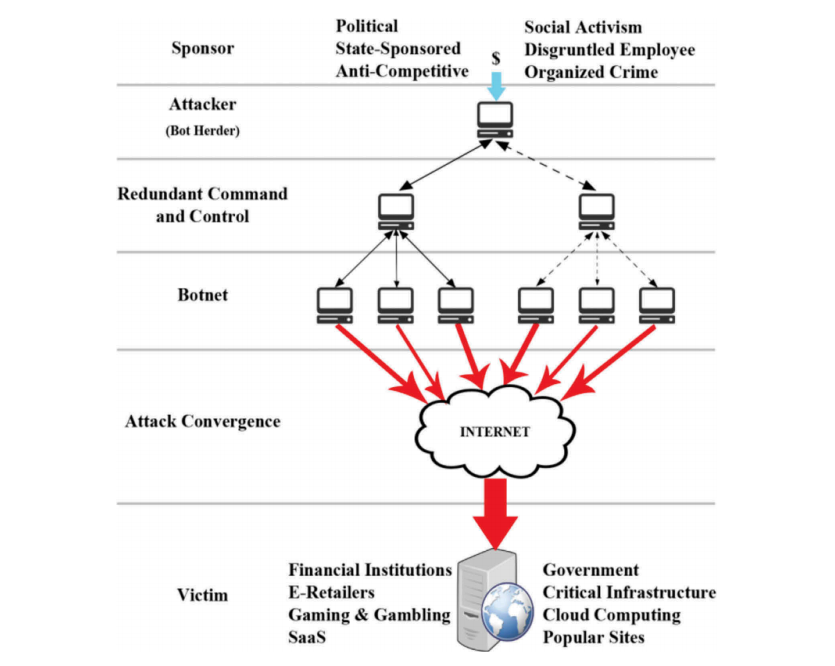
\includegraphics[width=\hsize]{images/introduzione/struttura_botnets_2.png}
    \caption{Struttura di lancio di attacchi DDoS \cite{ddos_survey_4}}
    \centering
\end{figure}



\section{Organizzazione della tesi}
